\documentclass[aspectratio=169]{beamer}
\usefonttheme[onlymath]{serif}

\usepackage[bahasa]{babel}
\usepackage[utf8]{inputenc}
\usepackage[mode=buildnew]{standalone}
\usepackage{algpseudocode}
\usepackage{algorithm}

\usepackage[style=apa]{biblatex}
\usepackage{mathtools}
\renewcommand*{\nameyeardelim}{\addcomma\addspace}
\addbibresource{references.bib}

\graphicspath{{resources/}}   % letak direktori penyimpanan gambar

\title[Modifikasi Adam]{Pengembangan dan Implementasi Modifikasi Pengoptimasi Adam pada Lingkungan Terdistribusi}
\author[]{
  Fransiskus Febryan Suryawan\\
  13519124
}
\institute{Institut Teknologi Bandung}
\date{}

\usetheme{venti}

\begin{document}

{
\makeatletter
\setlength{\hoffset}{-.5\beamer@sidebarwidth}
\setlength{\voffset}{-.2em}
\makeatother
\begin{frame}[plain]
  \titlepage
\end{frame}
}

\section*{Outline}
\begin{frame}{Outline}
  \begin{center}
    \tableofcontents
  \end{center}
\end{frame}

\section{Pendahuluan}
\subsection{Latar Belakang}
\begin{frame}{Deep Learning}
  \begin{center}
    \includestandalone[height=6em]{figures/dnn}
  \end{center}
  \begin{itemize}
    \item Deep Learning banyak digunakan dalam banyak domain
    \item Sebuah model Deep Learning memiliki parameter yang dapat dipelajari
    \item Pembelajaran pada Deep Learning banyak menggunakan \textit{backpropagation} untuk pembelajaran
    \item Pengoptimasi untuk pembelajaran: SGD, \textbf{Adam}, RMSProp, ...
    \item Arah perkembangan model Deep Learning umumnya adalah memperbanyak parameter untuk mendapat hasil yang lebih baik
  \end{itemize}
\end{frame}

\begin{frame}{Pengoptimasi Adam}
  \begin{enumerate}
    \item Pengoptimasi digunakan untuk mempelajari parameter pada model
    \item Adam \parencite{ADAMKingma} menggunakan \textit{learning rate} adaptif untuk setiap parameter
    \item Adam menggunakan estimasi momen orde pertama dan kedua untuk membantu pembelajaran
    \item Terdapat modifikasi Adam untuk pembelajaran model Deep Learning Terdistribusi
          \begin{itemize}
            \item CADA: Communication Adaptive Distributed Adam - pengurangan komunikasi \parencite{Chen2021CADA}
            \item Efficient-Adam: kompresi bobot menggunakan kuantisasi \parencite{Chen2022Efficient}
          \end{itemize}
    \item Belum ada modifikasi Adam yang mengurangi komunikasi serta melakukan kuantisasi secara bersamaan
  \end{enumerate}
\end{frame}

\begin{frame}{Deep Learning Terdistribusi}
  \begin{itemize}
    \item Model umum yang digunakan dalam distributed Deep Learning: \textbf{Parameter Server}
    \item Beberapa mesin dapat digunakan secara bersamaan untuk mempercepat pembelajaran model Deep Learning
    \item \textit{Bottleneck}: batasan \textit{bandwidth}
    \item Terdapat usaha untuk mengurangi kebutuhan \textit{bandwidth} untuk bertukar parameter selama pembelajaran
          \begin{itemize}
            \item Kompresi: \textit{lossless}, \textit{lossy}
            \item Pengurangan komunikasi
          \end{itemize}
  \end{itemize}
\end{frame}

\subsection{Rumusan Masalah}
\begin{frame}{Tujuan}
  \begin{itemize}
    \item Menggabungkan teknik pada CADA dengan Efficient-Adam
    \item Membandingkan hasil modifikasi yang telah dibuat dengan CADA
    \item Membandingkan hasil modifikasi yang dibuat dengan Efficient-Adam
  \end{itemize}
\end{frame}

\section{Penelitian Terkait}
\subsection{CADA}
\begin{frame}{CADA \parencite{Chen2021CADA}}
  \begin{itemize}
    \item Terdapat teknik \textit{Lazily Aggregated Gradient} \parencite{Chen2018LAG}
          \begin{itemize}
            \item Keefektifannya berkurang seiring berjalannya pembelajaran
          \end{itemize}
    \item Pengurangan komunikasi berdasarkan kriteria tertentu
    \item Memilih \textit{worker} yang akan memperbarui parameter
          \begin{itemize}
            \item CADA 1
                  \begin{equation*}
                    \| \delta_m^k - \tilde{\delta}_m^{k-\tau_m^k} \|^2 \le \frac{c}{d_{\mathrm{max}}}\sum_{d=1}^{d_{\mathrm{max}}}\| \theta^{k+1-d} - \theta^{k-d} \|^2
                  \end{equation*}
            \item CADA 2
                  \begin{equation*}
                    \| \nabla \ell (\theta^k; \xi_m^k) - \nabla \ell (\theta_m^{k-\tau_m^k}; \xi_m^k) \|^2 \le \frac{c}{d_{\mathrm{max}}} \sum_{d=1}^{d_{\mathrm{max}}} \| \theta^{k+1-d} - \theta^{k-d} \|^2
                  \end{equation*}
          \end{itemize}
  \end{itemize}
\end{frame}

\subsection{Efficient-Adam}
\begin{frame}{Efficient-Adam \parencite{Chen2022Efficient}}
  \begin{itemize}
    \item Kuantisasi untuk mengurangi ukuran parameter serta gradien
          \begin{itemize}
            \item Mengakibatkan presisi turun, mungkin terjadi bias
          \end{itemize}
    \item Error-feedback digunakan untuk mengurangi efek bias
  \end{itemize}
\end{frame}

\section{Rancangan Solusi}
\begin{frame}{Rancangan Solusi}
  \begin{itemize}
    \item Mendesain modifikasi Adam yang menggabungkan CADA \parencite{Chen2021CADA} dan Efficient-Adam \parencite{Chen2022Efficient}
          \begin{itemize}
            \item Harapan: Mengurangi kebutuhan \textit{bandwidth} lebih jauh
          \end{itemize}
    \item Menggunakan pustaka \texttt{PyTorch} untuk abstraksi model Parameter Server serta pembangunan model Deep Learning
          \begin{itemize}
            \item Model yang akan digunakan untuk evaluasi: ResNet20
            \item Dataset yang akan digunakan: CIFAR10
          \end{itemize}
    \item Jumlah komunikasi serta ukuran gradien akan dibandingkan antar teknik
  \end{itemize}
\end{frame}
\section{Implementasi dan Pengujian}
\begin{frame}{Implementasi}
  \begin{itemize}
    \item Implementasi dilakukan untuk teknik CADA, Efficient-Adam, dan teknik gabungan dari keduanya
    \item Implementasi dilakukan terpisah, dengan membangun sebuah kelas dasar yang diimplementasikan ketiganya
    \item Menggunakan arsitektur parameter server dengan memanfaatkan pustaka RPC pada \texttt{PyTorch}
  \end{itemize}
\end{frame}

\subsection{Algoritma}
\begin{frame}{Algoritma Parameter Server}
  \begin{algorithm}[H]
    \caption{Algoritma Parameter Server}
    \begin{algorithmic}[1]
      \State \textbf{Parameter:} Fungsi Kuantisasi $\mathcal{Q}_s$
      \State \textbf{Inisialisasi} vektor parameter $\theta_0$, error term $e_1 \gets 0$
      \State Sebarkan $\theta_0$ ke semua \textit{worker}
      \For{$t = 1,2,\dots,T$}
      \State $\hat{\delta_t} \gets \textnormal{rata-rata } \delta_t^{(i)}$ dari setiap \textit{worker}
      \State Sebarkan $\tilde{\delta_t} \gets \mathcal{Q}(\hat{\delta_t} + e_t)$
      \State $e_{t+1} \gets e_{t}$
      \State $\theta_{t+1} \gets \theta_t - \tilde{\delta_t}$
      \EndFor
    \end{algorithmic}
  \end{algorithm}
\end{frame}

\begin{frame}{Algoritma Worker}
  \begin{algorithm}[H]
    \caption{Modifikasi Adam untuk Worker ke-$i$}
    \begin{algorithmic}[1]
      \State \textbf{Parameter:} Fungsi Kuantisasi $\mathcal{Q}_w$, Hyperparameter Adam $\alpha, \beta_1, \beta_2$, konstanta batas $c$, batas maksimum penundaan $D$
      \State $m_0^{(i)} \gets 0, v_0^{(i)} \gets \epsilon, e_1^{(i)} \gets 0, \tau^{(i)} \gets 0$
      \State $\theta^{(i)}_0 \gets \theta_1$ dari server
      \For{$t=1,2,\dots,T$}
      \State $g_t^{(i)} \gets \nabla_\theta f_t(\theta_{t})$
      \State $v_t^{(i)} \gets \theta_t v_{t-1}^{(i)} + (1-\theta_t)[g_t^{(i)}]^2$
      \State $m_t^{(i)} \gets \beta_1 m_{t-1}^{(i)} + (1-\beta_1)g_t^{(i)}$
      \State $\alpha_t \gets \alpha \sqrt{1-\beta_2^t}/(1-\beta_1^t)$
      \State $\delta^{(i)} \gets \alpha_t m_t^{(i)}/\sqrt{v_t^{(i)}}+e_t^{(i)}$
      \State $\theta_t \gets \theta_{t-1} - \delta^{(i)}$
      \algstore{worker}
    \end{algorithmic}
  \end{algorithm}
\end{frame}

\begin{frame}{Algoritma Worker}
  \begin{algorithm}[H]
    \begin{algorithmic}[1]
      \algrestore{worker}
      \State Hitung $\nabla f_t(\theta^{(i)}_{t})$ dan $\nabla f_t(\theta^{(i)}_{t-\tau})$
      \State $\delta^{(i)} \gets \mathcal{Q}_w(\delta^{(i)})$
      \If{Kondisi \ref{cada2cond} tidak terpenuhi atau $\tau \ge D$}
      \State Kirim $\delta^{(i)}$
      \State $\tau \gets 1$
      \Else
      \State $\tau \gets \tau + 1$
      \EndIf
      \State $e_{t+1}^{(i)} \gets \alpha_t \frac{m_t^{(i)}}{\sqrt{v_t^{(i)}}} + e_t^{(i)} - \delta_t^{(i)}$
      \State Terima $\tilde{\delta_t}$ dari server
      \State $\theta_{t} \gets \theta_{t-1} - \tilde{\delta_t}$
      \EndFor
    \end{algorithmic}
  \end{algorithm}
\end{frame}

\begin{frame}{Kondisi Worker}
  \begin{equation}
    \label{cada2cond}
    \|\nabla f_t(\theta_t) - \nabla f_t(\theta_{t-\tau})\|^2 \leq \frac{c}{D} \sum_{d=1}^{D} \|\theta_{t+1-d} - \theta_{t-d}\|^2
  \end{equation}
\end{frame}

\subsection{Lingkungan Pengujian}
\begin{frame}{Lingkungan Pengujian}
  Pengujian dilakukan pada server DGX, menggunakan satu GPU yang dialokasikan.

  \begin{table}
    \caption{Spesifikasi Server DGX}
    \centering
    \begin{tabular}[ht]{ | c | c | }
      \hline
      \textbf{Parameter} & \textbf{Spesifikasi}                           \\
      \hline
      CPU                & 2x Intel Xeon E5-2698 v3 (16-core, Haswell-EP) \\
      \hline
      RAM                & 512GB DDR4-2133                                \\
      \hline
      GPU                & 8x Tesla V100 32GB VRAM                        \\
      \hline
      Penyimpanan        & 4x1.92 TB SSD                                  \\
      \hline
    \end{tabular}
  \end{table}
\end{frame}

\begin{frame}{Lingkungan Pengujian}
  Versi kakas dan pustaka yang digunakan dalam pengujian
  \begin{table}
    \caption{Versi Perangkat Lunak}\label{softwares}
    \centering
    \begin{tabular}{ | c | c | }
      \hline
      \textbf{Perangkat Lunak} & \textbf{Versi} \\
      \hline
      Python                   & 3              \\
      \hline
      PyTorch                  & 1.13.1+cuda    \\
      \hline
      TorchVision              & 0.14.1+cuda    \\
      \hline
    \end{tabular}
  \end{table}
\end{frame}

\subsection{Skenario Pengujian}
\begin{frame}{Skenario Pengujian}
  \begin{itemize}
    \item Pengujian dilakukan dengan melatih ResNet20 pada dataset CIFAR10
    \item Pelatihan dilakukan dengan membagi data ke 10 \textit{worker} yang dijalankan dalam 1 GPU
    \item Jumlah komunikasi, jumlah byte yang digunakan, serta akurasi model akan dicatat setiap \textit{epoch}
  \end{itemize}
\end{frame}
\begin{frame}{Skenario Pengujian}
  \begin{columns}[b]
    \begin{column}{3.5cm}
      Hyperparameter untuk CADA \\
      \begin{tabular}{ | c | c | }
        \hline
        \textbf{Parameter} & \textbf{Nilai} \\
        \hline
        $\alpha$           & 0.01           \\
        \hline
        $\beta_1$          & 0.9            \\
        \hline
        $\beta_2$          & 0.99           \\
        \hline
        $D$                & 50             \\
        \hline
        $d_{max}$          & 2              \\
        \hline
        $c$                & 0.12           \\
        \hline
      \end{tabular}
    \end{column}
    \begin{column}{3.5cm}
      Hyperparameter untuk Efficient-Adam \\
      \begin{tabular}{ | c | c | }
        \hline
        \textbf{Parameter} & \textbf{Nilai} \\
        \hline
        $\alpha$           & 0.0005         \\
        \hline
        $\beta_1$          & 0.9            \\
        \hline
        $\beta_2$          & 0.999          \\
        \hline
      \end{tabular}
    \end{column}
    \begin{column}{3.5cm}
      Hyperparameter untuk gabungan \\
      \begin{tabular}{ | c | c | }
        \hline
        \textbf{Parameter} & \textbf{Nilai} \\
        \hline
        $\alpha$           & 0.0005         \\
        \hline
        $\beta_1$          & 0.9            \\
        \hline
        $\beta_2$          & 0.999          \\
        \hline
        $D$                & 50             \\
        \hline
        $d_{max}$          & 2              \\
        \hline
        $c$                & 0.12           \\
        \hline
      \end{tabular}
    \end{column}
  \end{columns}
\end{frame}

\subsection{Hasil Pengujian}
\begin{frame}{Hasil Pengujian}
  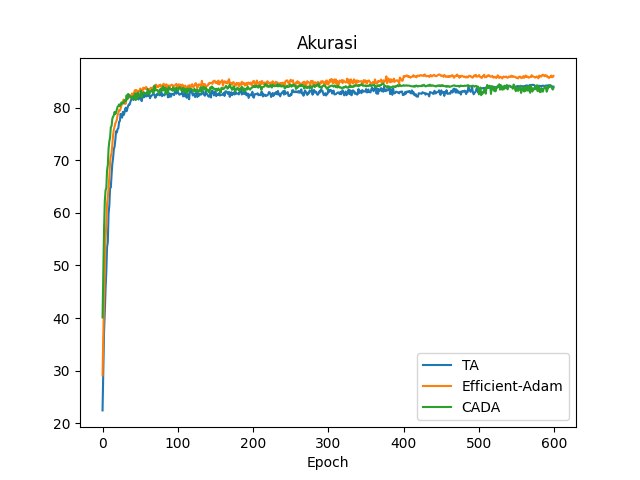
\includegraphics[width=6.5cm]{acc.png}
  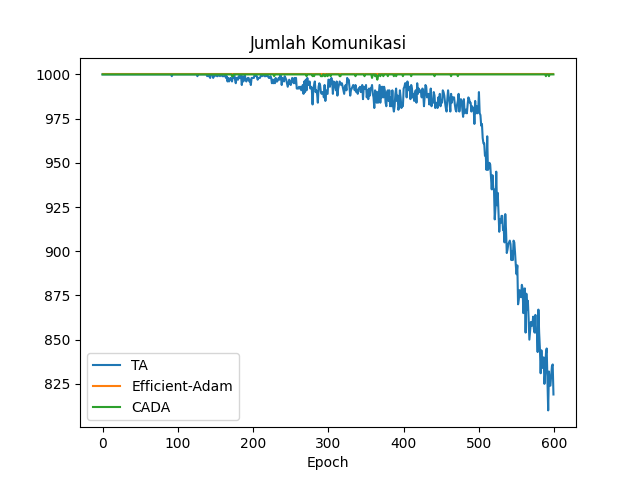
\includegraphics[width=6.5cm]{comms.png}
\end{frame}

\begin{frame}{Hasil Pengujian}
  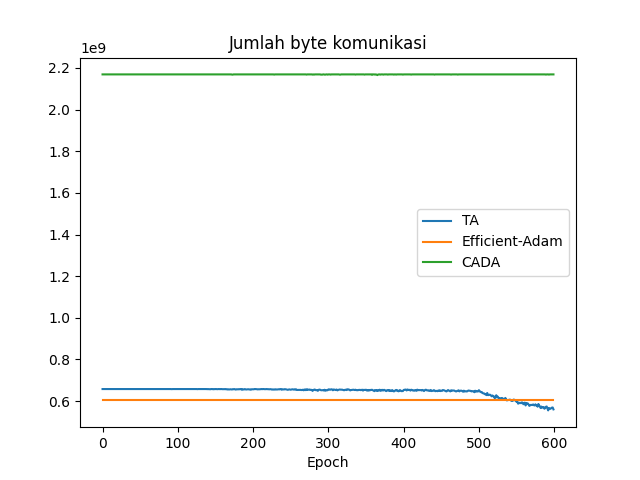
\includegraphics[width=7cm]{bits.png}
\end{frame}

\subsection{Analisis Hasil Pengujian}
\begin{frame}{Analisis Hasil Pengujian}
  \begin{itemize}
    \item Akurasi didapatkan saling mendekati (sekitar 84\%-86\%)
    \item Jumlah komunikasi yang dilakukan paling sedikit dari teknik gabungan (lebih sedikit 13.383 dibandingkan Efficient-Adam)
    \item Jumlah bytes yang digunakan paling sedikit oleh Efficient-Adam (0.303 kali CADA), namun teknik gabungan berkurang tiap epoch dimulai sekitar epoch 500
  \end{itemize}
\end{frame}

\end{document}
